\documentclass[11pt,a4paper]{article}
\usepackage[utf8]{inputenc}
\usepackage[T1]{fontenc}
%nobabel
\usepackage{mathpazo}
\usepackage{amsmath,amssymb,amsthm,mathtools}
\usepackage{bm}
\usepackage[margin=2.3cm,top=2.5cm,bottom=2.5cm]{geometry}
\usepackage{microtype}
\usepackage{xcolor}
\usepackage{booktabs,array,tabularx}
\usepackage{enumitem}
\usepackage{fancyhdr}
\usepackage{titlesec}
\usepackage[most]{tcolorbox}
\usepackage{pgfplots}
\usepgfplotslibrary{polar}
\pgfplotsset{compat=1.17}
\usepackage[colorlinks=true,linkcolor=linkblue,citecolor=linkblue,urlcolor=linkblue]{hyperref}

\definecolor{boxblue}{RGB}{66,96,150}
\definecolor{linkblue}{RGB}{40,90,170}
\definecolor{secblue}{RGB}{60,100,170}
\definecolor{boxback}{RGB}{245,247,252}
\definecolor{warnred}{RGB}{170,50,50}
\definecolor{warnback}{RGB}{253,245,245}

\titleformat{\section}{\normalfont\Large\bfseries\color{secblue}}{\thesection}{1em}{}
\titleformat{\subsection}{\normalfont\large\bfseries}{\thesubsection}{1em}{}

\pagestyle{fancy}
\fancyhf{}
\fancyhead[L]{\small Funciones de Green, Liénard--Wiechert y radiación}
\fancyhead[R]{\small Guía de estudio -- Quiz 5}
\fancyfoot[C]{\thepage}
\renewcommand{\headrulewidth}{0.4pt}

\newtcolorbox{resbox}[1]{enhanced,breakable,colback=boxback,colframe=boxblue,
  coltitle=white,fonttitle=\bfseries,title={#1},arc=2mm,boxrule=0.6pt,
  left=2mm,right=2mm,top=1mm,bottom=1mm}
\newtcolorbox{warnbox}[1]{enhanced,breakable,colback=warnback,colframe=warnred,
  coltitle=white,fonttitle=\bfseries,title={#1},arc=2mm,boxrule=0.6pt}
\newtcolorbox{refbox}{enhanced,colback=white,colframe=boxblue,arc=2mm,boxrule=0.6pt,
  left=3mm,right=3mm}

\newcounter{ejer}
\newcommand{\ejercicio}[1]{\refstepcounter{ejer}%
  \subsection*{Ej.~\theejer\ -- #1}\addcontentsline{toc}{subsection}{Ej.~\theejer\ -- #1}}
\newcommand{\sol}{\par\noindent\textit{Solución.}\ }

\newcommand{\Rv}{\bm{\mathcal R}}
\newcommand{\Rs}{\mathcal R}
\newcommand{\Rh}{\hat{\bm{\mathcal R}}}
\newcommand{\nh}{\hat{\mathbf n}}
\newcommand{\bv}{\mathbf v}
\newcommand{\av}{\mathbf a}
\newcommand{\uv}{\mathbf u}
\newcommand{\rr}{\mathbf r}
\newcommand{\dd}{\mathrm d}
\newcommand{\boxop}{\Box^2}
\newcommand{\bbeta}{\bm\beta}

\theoremstyle{remark}
\newtheorem*{demo}{Demostración}

\setlength{\parindent}{0pt}
\setlength{\parskip}{0.5em}

\renewcommand{\contentsname}{Índice}
\begin{document}

% ================= PORTADA =================
\begin{titlepage}
\thispagestyle{empty}
\centering
\vspace*{3.2cm}
{\Huge\bfseries Funciones de Green\\[0.25em] y Radiación Electromagnética\par}
\vspace{1.2em}
{\Large Guía de estudio detallada -- Quiz 5\par}
\vspace{1.5em}
{\large Ecuación de onda $\cdot$ Potenciales retardados $\cdot$ Liénard--Wiechert\\
Fórmulas de Larmor y Liénard $\cdot$ Aceleración $\parallel$ y $\perp$ a $\mathbf v$ $\cdot$ Radiación dipolar\par}
\vspace{2.5em}
\begin{minipage}{0.82\textwidth}
\begin{refbox}
\textbf{Bibliografía base}
\begin{itemize}[leftmargin=1.2em,itemsep=0.3em]
\item D. J. Griffiths, \textit{Introduction to Electrodynamics}, 4.ª ed.: Secs. \textbf{10.1--10.3}
(potenciales, retardo, Liénard--Wiechert) y \textbf{11.1--11.2} (radiación dipolar, cargas puntuales,
reacción de radiación).
\item J. D. Jackson, \textit{Classical Electrodynamics}, 3.ª ed.: Secs. \textbf{6.2--6.5}
(potenciales, gauge, \textbf{funciones de Green de la ecuación de onda}, Jefimenko), \textbf{9.1--9.3}
(radiación multipolar) y \textbf{14.1--14.3} (Liénard--Wiechert, Larmor, distribución angular).
\end{itemize}
\end{refbox}
\end{minipage}
\vspace{2em}

{\large Electromagnetismo Intermedio -- Licenciatura en Física\\ Universidad de Valparaíso, II Semestre 2026\par}
\vfill
{\small Las integrales angulares de las Secs.~6.4--6.5 fueron verificadas simbólicamente con \texttt{sympy};
los valores numéricos de los ejercicios se recalcularon con constantes CODATA.\par}
\end{titlepage}

\tableofcontents
\newpage

% ================= 1 =================
\section{Cómo usar esta guía}

El quiz 5 (17-11) cubre el bloque de las clases 22--26: soluciones de Maxwell en términos de
potenciales, transformaciones de gauge, gauge de Lorenz, \textbf{funciones de Green de la ecuación
de onda}, potenciales de Liénard--Wiechert, campos de una carga arbitraria, radiación dipolar y
potencia radiada con aceleración paralela y perpendicular a la velocidad. La guía tiene tres bloques:
\begin{enumerate}[itemsep=0.2em]
\item \textbf{Teoría} (Secs.~2--8): cada resultado se deriva sin saltar pasos algebraicos.
\item \textbf{Recetario} (Sec.~9): qué herramienta usar, trucos y errores frecuentes.
\item \textbf{Ejercicios} (Secs.~10--11): resueltos paso a paso y propuestos con respuesta.
\end{enumerate}

Los apuntes del curso (\texttt{Funciones\_de\_green.pdf}) desarrollan el caso electrostático,
$\nabla^2G=-4\pi\delta^{(3)}$. Esta guía es su extensión natural al caso dependiente del tiempo:
el operador $\nabla^2$ se reemplaza por $\boxop$ y la fuente puntual pasa a ser un evento en el
espacio-tiempo.

\subsection{Mapa de referencias}

\begin{center}
\renewcommand{\arraystretch}{1.25}
\begin{tabularx}{\textwidth}{>{\raggedright}p{5.2cm}>{\raggedright}X>{\raggedright\arraybackslash}X}
\toprule
\textbf{Tema} & \textbf{Griffiths (4.ª ed.)} & \textbf{Jackson (3.ª ed.)}\\
\midrule
Potenciales, gauge de Coulomb y Lorenz & Sec. 10.1 & Secs. 6.2--6.3\\
Función de Green de la ecuación de onda & (implícita en 10.2.1) & Sec. 6.4 (ecs. 6.40--6.48)\\
Potenciales retardados & Sec. 10.2.1 (ec. 10.26) & Sec. 6.4 (ec. 6.48)\\
Ecuaciones de Jefimenko & Sec. 10.2.2 & Sec. 6.5\\
Liénard--Wiechert & Sec. 10.3.1 (ecs. 10.46--10.47) & Sec. 14.1 (ec. 14.8)\\
Campos de carga arbitraria & Sec. 10.3.2 (ecs. 10.72--10.73) & Sec. 14.1 (ecs. 14.13--14.14)\\
Radiación dipolar eléctrica y magnética & Secs. 11.1.2--11.1.4 & Secs. 9.2--9.3\\
Larmor, Liénard & Sec. 11.2.1 (ecs. 11.70, 11.74) & Sec. 14.2 (ecs. 14.22, 14.26)\\
Distribución angular ($\parallel$, $\perp$) & Ej. 11.3; Prob. 11.15 & Sec. 14.3 (ecs. 14.39, 14.44)\\
Reacción de radiación & Sec. 11.2.2 & Cap. 16\\
\bottomrule
\end{tabularx}
\end{center}

\subsection{Convenciones (¡léelas antes de mezclar libros!)}

\begin{warnbox}{Diferencias de notación entre Griffiths y Jackson}
\begin{itemize}[itemsep=0.2em,leftmargin=1.2em]
\item \textbf{Unidades:} todo en SI. Jackson usa SI en los Caps.~1--10 y \emph{gaussianas} desde el
Cap.~11: para pasar de gaussianas a SI en el Cap.~14, $q^2\to q^2/(4\pi\varepsilon_0)$.
\item \textbf{Vector de separación:} Griffiths usa la ``r cursiva''; aquí se escribe
$\Rv=\rr-\rr'$ (o $\Rv=\rr-\mathbf w(t_r)$ para una carga puntual), $\Rs=|\Rv|$, $\nh\equiv\Rh$.
\item \textbf{Normalización de $G$:} se sigue a Jackson, $\boxop G=-4\pi\delta^{(3)}\delta$, igual
que en los apuntes del curso. Con ella, $G\to1/R$ en el límite estático.
\item \textbf{Fourier:} $g(t)=\frac1{2\pi}\int g(\omega)e^{-i\omega t}\dd\omega$,\quad
$g(\omega)=\int g(t)e^{i\omega t}\dd t$.\quad Así $\partial_t\to-i\omega$.
\item \textbf{Relatividad:} $\bbeta=\bv/c$, $\gamma=(1-\beta^2)^{-1/2}$; métrica $(-,+,+,+)$.
\end{itemize}
\end{warnbox}

% ================= 2 =================
\section{Potenciales, gauge y ecuaciones de onda}

Como $\nabla\cdot\mathbf B=0$, se escribe $\mathbf B=\nabla\times\mathbf A$. Sustituyendo en la ley
de Faraday, $\nabla\times(\mathbf E+\partial_t\mathbf A)=0$, de modo que
\begin{equation}
\mathbf E=-\nabla V-\frac{\partial\mathbf A}{\partial t}.
\label{eq:EAV}
\end{equation}

\textbf{Ley de Gauss.} $\nabla\cdot\mathbf E=\rho/\varepsilon_0$ con \eqref{eq:EAV}:
\begin{equation}
\nabla^2V+\frac{\partial}{\partial t}(\nabla\cdot\mathbf A)=-\frac{\rho}{\varepsilon_0}.
\label{eq:gaussV}
\end{equation}

\textbf{Ley de Ampère--Maxwell.} $\nabla\times\mathbf B=\mu_0\mathbf J+\mu_0\varepsilon_0\partial_t\mathbf E$,
con $\nabla\times(\nabla\times\mathbf A)=\nabla(\nabla\cdot\mathbf A)-\nabla^2\mathbf A$ y
$\mu_0\varepsilon_0=1/c^2$:
\begin{align}
\nabla(\nabla\cdot\mathbf A)-\nabla^2\mathbf A
&=\mu_0\mathbf J-\frac1{c^2}\nabla\frac{\partial V}{\partial t}-\frac1{c^2}\frac{\partial^2\mathbf A}{\partial t^2}\nonumber\\
\Rightarrow\quad
\left(\nabla^2\mathbf A-\frac1{c^2}\frac{\partial^2\mathbf A}{\partial t^2}\right)
-\nabla\!\left(\nabla\cdot\mathbf A+\frac1{c^2}\frac{\partial V}{\partial t}\right)&=-\mu_0\mathbf J.
\label{eq:ampA}
\end{align}

\begin{resbox}{Transformaciones de gauge}
Para cualquier función escalar $\lambda(\rr,t)$,
\[
\mathbf A'=\mathbf A+\nabla\lambda,\qquad V'=V-\frac{\partial\lambda}{\partial t}
\]
deja $\mathbf E$ y $\mathbf B$ invariantes: $\nabla\times\nabla\lambda=0$ y
$-\nabla(-\partial_t\lambda)-\partial_t(\nabla\lambda)=0$.
\end{resbox}

\textbf{Gauge de Coulomb}, $\nabla\cdot\mathbf A=0$: \eqref{eq:gaussV} se vuelve Poisson,
$\nabla^2V=-\rho/\varepsilon_0$. Así $V$ responde \emph{instantáneamente} a $\rho$, lo que no viola la
causalidad porque $V$ no es observable: el retardo reaparece en $\mathbf A$.

\textbf{Gauge de Lorenz}, $\nabla\cdot\mathbf A+\frac1{c^2}\partial_tV=0$. Siempre es alcanzable: si
$(\mathbf A,V)$ no lo cumplen, basta elegir $\lambda$ con
\[
\boxop\lambda=-\Big(\nabla\cdot\mathbf A+\tfrac1{c^2}\partial_tV\Big),
\]
que es otra ecuación de onda con fuente (se resuelve con la misma $G$ de la Sec.~3). Queda una
libertad residual: cualquier $\lambda$ con $\boxop\lambda=0$.

En el gauge de Lorenz, el gradiente en \eqref{eq:ampA} se anula y en \eqref{eq:gaussV}
$\partial_t(\nabla\cdot\mathbf A)=-c^{-2}\partial_t^2V$:
\begin{resbox}{Ecuaciones de onda inhomogéneas (gauge de Lorenz)}
\begin{equation}
\boxop V=-\frac{\rho}{\varepsilon_0},\qquad \boxop\mathbf A=-\mu_0\mathbf J,\qquad
\boxop\equiv\nabla^2-\frac1{c^2}\frac{\partial^2}{\partial t^2}.
\label{eq:ondas}
\end{equation}
Cuatro ecuaciones \emph{desacopladas}, todas con la misma estructura: un problema de Green.
\end{resbox}

% ================= 3 =================
\section{Función de Green de la ecuación de onda (Jackson §6.4)}

Las cuatro ecuaciones \eqref{eq:ondas} tienen la forma genérica
\begin{equation}
\nabla^2\Psi-\frac1{c^2}\frac{\partial^2\Psi}{\partial t^2}=-4\pi f(\mathbf x,t),
\label{eq:generica}
\end{equation}
con $f=\rho/(4\pi\varepsilon_0)$ para $V$ y $f=\mu_0J_i/(4\pi)$ para cada $A_i$. La función de Green
es la respuesta a un \emph{evento} puntual:
\begin{equation}
\left(\nabla^2-\frac1{c^2}\partial_t^2\right)G(\mathbf x,t;\mathbf x',t')=-4\pi\,\delta^{(3)}(\mathbf x-\mathbf x')\,\delta(t-t').
\label{eq:defG}
\end{equation}

\subsection{Paso 1: Fourier en el tiempo $\Rightarrow$ Helmholtz}

Con $\partial_t^2\to-\omega^2$ y $k\equiv\omega/c$, la transformada de \eqref{eq:generica} es
\begin{equation}
(\nabla^2+k^2)\Psi(\mathbf x,\omega)=-4\pi f(\mathbf x,\omega),
\end{equation}
cuya función de Green satisface
\begin{equation}
(\nabla^2+k^2)G_k(\mathbf x,\mathbf x')=-4\pi\,\delta^{(3)}(\mathbf x-\mathbf x').
\label{eq:helm}
\end{equation}

\subsection{Paso 2: resolver Helmholtz en espacio libre}

Sin fronteras no hay dirección privilegiada, así que $G_k=G_k(R)$ con $R=|\mathbf x-\mathbf x'|$.
Para $R\neq0$, usando el laplaciano radial $\nabla^2g=\frac1R\frac{\dd^2}{\dd R^2}(Rg)$:
\[
\frac1R\frac{\dd^2}{\dd R^2}(RG_k)+k^2G_k=0
\quad\Longrightarrow\quad
\frac{\dd^2}{\dd R^2}(RG_k)+k^2(RG_k)=0
\quad\Longrightarrow\quad
RG_k=A\,e^{ikR}+B\,e^{-ikR}.
\]
\textbf{Normalización.} Cerca de $R=0$, $kR\ll1$ y $G_k\to(A+B)/R$. Como
$\nabla^2(1/R)=-4\pi\delta^{(3)}$, la delta de \eqref{eq:helm} se reproduce si $A+B=1$. El término
$k^2G_k\sim k^2/R$ no contribuye: integrado sobre una bola de radio $\epsilon$,
$\int k^2R^{-1}\,4\pi R^2\dd R=2\pi k^2\epsilon^2\to0$. Las dos soluciones independientes son
\begin{equation}
G_k^{(\pm)}(R)=\frac{e^{\pm ikR}}{R}.
\end{equation}

\subsection{Paso 3: volver al dominio temporal}

La transformada de $\delta(t-t')$ es $e^{i\omega t'}$, por lo que $G(\omega)=G_k\,e^{i\omega t'}$.
Invirtiendo, con $\tau\equiv t-t'$:
\begin{equation}
G^{(\pm)}=\frac1{2\pi}\int_{-\infty}^{\infty}\dd\omega\,\frac{e^{\pm i\omega R/c}}{R}\,e^{-i\omega\tau}
=\frac1R\,\frac1{2\pi}\int_{-\infty}^{\infty}\dd\omega\,e^{-i\omega(\tau\mp R/c)}
=\frac{\delta(\tau\mp R/c)}{R}.
\end{equation}

\begin{resbox}{Función de Green retardada (Jackson ec. 6.44)}
\begin{equation}
G^{(+)}(\mathbf x,t;\mathbf x',t')=\frac{\delta\!\left(t'-\left[t-\dfrac{|\mathbf x-\mathbf x'|}{c}\right]\right)}{|\mathbf x-\mathbf x'|}
\label{eq:Gret}
\end{equation}
Es una cáscara esférica que se expande desde $\mathbf x'$ con rapidez $c$ y amplitud $1/R$. Se anula
para $t<t'$: \textbf{respeta la causalidad}. La avanzada, $G^{(-)}=\delta(t'-[t+R/c])/R$, es solución
matemática pero describe un efecto anterior a su causa; se descarta por condición de contorno
(no hay radiación entrante desde el infinito).
\end{resbox}

\subsection{Vista 4D: contornos y propagadores}

Transformando en las cuatro coordenadas,
$G=\int\frac{\dd^3k\,\dd\omega}{(2\pi)^4}\tilde G\,e^{i(\mathbf k\cdot\mathbf R-\omega\tau)}$, la ec.
\eqref{eq:defG} da $(-k^2+\omega^2/c^2)\tilde G=-4\pi$:
\begin{equation}
\tilde G(\mathbf k,\omega)=\frac{4\pi}{k^2-\omega^2/c^2},\qquad\text{polos en }\omega=\pm ck.
\end{equation}
La integral en $\omega$ está mal definida hasta elegir cómo rodear los polos. La prescripción
\textbf{retardada} los baja: $\omega\to\omega+i\epsilon$, es decir, polos en $\pm ck-i\epsilon$. Si
$\tau<0$, $e^{-i\omega\tau}$ decae en el semiplano superior; cerrando por arriba no se encierra ningún
polo y $G=0$. Para $\tau>0$ se cierra por abajo, se recogen ambos polos y se recupera
\eqref{eq:Gret}. Esta es exactamente la lógica de los propagadores retardado, avanzado y de Feynman en
QFT.

\subsection{Límite estático: conexión con los apuntes}

Si $f$ no depende del tiempo, $\int\dd t'\,\delta(t'-t+R/c)=1$ y
$\Psi=\int f(\mathbf x')/|\mathbf x-\mathbf x'|\,\dd^3x'$: se recupera la función de Green de Poisson
$G=1/R$ con $\nabla^2G=-4\pi\delta^{(3)}$, la ec.~(12) de los apuntes del curso. El tiempo sólo añade
el \emph{retardo}.

% ================= 4 =================
\section{Potenciales retardados (Griffiths §10.2)}

Por superposición, $\Psi(\mathbf x,t)=\int\dd^3x'\dd t'\,G^{(+)}f(\mathbf x',t')$. La integral en $t'$
se hace con la delta:
\begin{equation}
\Psi(\mathbf x,t)=\int\frac{[f(\mathbf x',t')]_{\rm ret}}{|\mathbf x-\mathbf x'|}\dd^3x'.
\end{equation}

\begin{resbox}{Potenciales retardados}
\begin{equation}
V(\rr,t)=\frac1{4\pi\varepsilon_0}\int\frac{\rho(\rr',t_r)}{R}\dd\tau',\qquad
\mathbf A(\rr,t)=\frac{\mu_0}{4\pi}\int\frac{\mathbf J(\rr',t_r)}{R}\dd\tau',\qquad
t_r\equiv t-\frac{R}{c}.
\label{eq:retard}
\end{equation}
\end{resbox}

\begin{warnbox}{Cuidado: los campos no se ``retardan'' ingenuamente}
Retardar los potenciales es correcto; retardar Coulomb y Biot--Savart \emph{no}. Al derivar
\eqref{eq:retard}, $\nabla$ también actúa sobre $t_r$ y aparecen términos en $\dot\rho$ y $\dot{\mathbf J}$
(ecuaciones de Jefimenko, Griffiths 10.2.2 / Jackson 6.5):
\[
\mathbf E=\frac1{4\pi\varepsilon_0}\int\left[\frac{\rho}{R^2}\hat{\mathbf R}+\frac{\dot\rho}{cR}\hat{\mathbf R}-\frac{\dot{\mathbf J}}{c^2R}\right]_{t_r}\dd\tau',\qquad
\mathbf B=\frac{\mu_0}{4\pi}\int\left[\frac{\mathbf J}{R^2}+\frac{\dot{\mathbf J}}{cR}\right]_{t_r}\times\hat{\mathbf R}\,\dd\tau'.
\]
\end{warnbox}

% ================= 5 =================
\section{Potenciales de Liénard--Wiechert}

\subsection{Derivación con la función de Green (Jackson §14.1)}

Una carga puntual sobre la trayectoria $\mathbf w(t')$ tiene $\rho(\rr',t')=q\,\delta^{(3)}(\rr'-\mathbf w(t'))$.
Conviene \emph{no} integrar primero en $t'$:
\begin{align}
V(\rr,t)&=\frac1{4\pi\varepsilon_0}\int\dd t'\int\dd^3r'\,
\frac{q\,\delta^{(3)}(\rr'-\mathbf w(t'))\;\delta\!\left(t-t'-|\rr-\rr'|/c\right)}{|\rr-\rr'|}\nonumber\\
&=\frac{q}{4\pi\varepsilon_0}\int\dd t'\,\frac{\delta\big(g(t')\big)}{|\rr-\mathbf w(t')|},\qquad
g(t')\equiv t'+\frac{|\rr-\mathbf w(t')|}{c}-t.
\end{align}
\textbf{Punto clave:} $\delta(g(t'))=\delta(t'-t_r)/|g'(t_r)|$, con $g(t_r)=0$. Con
$\Rv=\rr-\mathbf w(t')$ y $\dd\mathbf w/\dd t'=\bv$:
\[
g'(t')=1+\frac1c\frac{\dd}{\dd t'}|\rr-\mathbf w(t')|=1+\frac1c\,\Rh\cdot(-\bv)=1-\frac{\Rh\cdot\bv}{c}>0.
\]
Por tanto, y análogamente con $\mathbf J=q\bv\,\delta^{(3)}$:
\begin{resbox}{Potenciales de Liénard--Wiechert}
\begin{equation}
V(\rr,t)=\frac1{4\pi\varepsilon_0}\,\frac{qc}{\Rs c-\Rv\cdot\bv},\qquad
\mathbf A(\rr,t)=\frac{\bv}{c^2}\,V(\rr,t),
\label{eq:LW}
\end{equation}
todo evaluado en el tiempo retardado $t_r$, definido por $c(t-t_r)=|\rr-\mathbf w(t_r)|$.
\end{resbox}
El factor $(1-\Rh\cdot\bbeta)^{-1}$ es puramente geométrico: una carga que se acerca ``parece'' más
extensa porque permanece más tiempo dentro del cono de luz pasado del observador (Griffiths, Fig.~10.6).

\subsection{Derivadas del tiempo retardado}

Hacen falta para calcular los campos. Se parte de $c(t-t_r)=\Rs=|\rr-\mathbf w(t_r)|$ y se define
\begin{equation}
\uv\equiv c\Rh-\bv.
\end{equation}

\textbf{Derivada temporal.} Derivando respecto de $t$:
\[
c\left(1-\frac{\partial t_r}{\partial t}\right)=\frac{\partial\Rs}{\partial t}=-\Rh\cdot\bv\,\frac{\partial t_r}{\partial t}
\quad\Longrightarrow\quad
\boxed{\frac{\partial t_r}{\partial t}=\frac{c}{c-\Rh\cdot\bv}=\frac{\Rs c}{\Rv\cdot\uv}}
\]

\textbf{Gradiente.} $-c\nabla t_r=\nabla\Rs$, y $\nabla\Rs$ tiene una parte explícita y otra a través
de $t_r$: $\nabla\Rs=\Rh-(\Rh\cdot\bv)\nabla t_r$. Luego
\[
-c\nabla t_r=\Rh-(\Rh\cdot\bv)\nabla t_r
\quad\Longrightarrow\quad
\nabla t_r\,(\Rh\cdot\bv-c)=\Rh
\quad\Longrightarrow\quad
\boxed{\nabla t_r=-\frac{\Rv}{\Rv\cdot\uv}}
\]

\subsection{Campos de una carga en movimiento arbitrario}

Con estas dos derivadas, $\mathbf E=-\nabla V-\partial_t\mathbf A$ y $\mathbf B=\nabla\times\mathbf A$
se obtienen por álgebra vectorial directa (Griffiths ecs. 10.72--10.73):
\begin{resbox}{Campos de Liénard--Wiechert}
\begin{equation}
\mathbf E(\rr,t)=\frac{q}{4\pi\varepsilon_0}\frac{\Rs}{(\Rv\cdot\uv)^3}
\Big[\underbrace{(c^2-v^2)\,\uv}_{\text{campo de velocidad}\,\sim\,1/\Rs^2}
+\underbrace{\Rv\times(\uv\times\av)}_{\text{campo de radiación}\,\sim\,1/\Rs}\Big],
\qquad
\mathbf B=\frac1c\,\Rh\times\mathbf E.
\label{eq:LWfields}
\end{equation}
\end{resbox}

\subsection{Carga con velocidad constante}

Con $\av=0$ y expresando todo en la posición \emph{presente} $\mathbf R_0=\rr-\bv t$, con $\theta$ el
ángulo entre $\mathbf R_0$ y $\bv$:
\begin{equation}
\mathbf E=\frac{q}{4\pi\varepsilon_0}\,\frac{1-v^2/c^2}{\left(1-\frac{v^2}{c^2}\sin^2\theta\right)^{3/2}}\,\frac{\hat{\mathbf R}_0}{R_0^2},
\qquad \mathbf B=\frac1{c^2}\,\bv\times\mathbf E.
\end{equation}
El campo apunta radialmente desde donde la carga \emph{está ahora}, aunque la información partió en
$t_r$, y se comprime en el plano $\perp\bv$ (la ``panqueca'' de Lorentz). Ver Ej.~\ref{ej:vconst}.

% ================= 6 =================
\section{Potencia radiada}

\subsection{Campo de radiación y vector de Poynting}

Lejos de la carga sólo sobrevive $\mathbf E_{\rm rad}\perp\Rh$. Con
$\mathbf B=\frac1c\Rh\times\mathbf E$ y $\mathbf E\cdot\Rh=0$:
\[
\mathbf S=\frac1{\mu_0}\mathbf E\times\Big(\frac1c\Rh\times\mathbf E\Big)
=\frac1{\mu_0c}\Big[\Rh\,E^2-\mathbf E\,(\mathbf E\cdot\Rh)\Big]
=\frac{E_{\rm rad}^2}{\mu_0c}\,\Rh.
\]
Como $S\propto1/\Rs^2$, la potencia a través de una esfera en el infinito es \emph{finita}: eso
\emph{define} la radiación. El campo de velocidad ($\propto1/\Rs^2$) da $S\propto1/\Rs^4$ y no contribuye.

\subsection{Fórmula de Larmor ($v=0$ instantáneo)}

Con $\uv=c\Rh$:
\[
\mathbf E_{\rm rad}=\frac{q}{4\pi\varepsilon_0c^2\Rs}\Big[\Rh\times(\Rh\times\av)\Big]
=\frac{\mu_0q}{4\pi\Rs}\Big[(\Rh\cdot\av)\Rh-\av\Big],\qquad
|\mathbf E_{\rm rad}|=\frac{\mu_0qa\sin\theta}{4\pi\Rs},
\]
\[
\frac{\dd P}{\dd\Omega}=\Rs^2S=\frac{\mu_0q^2a^2}{16\pi^2c}\sin^2\theta.
\]
Con $\int\sin^2\theta\,\dd\Omega=2\pi\int_{-1}^1(1-x^2)\dd x=\frac{8\pi}{3}$:
\begin{resbox}{Fórmula de Larmor}
\begin{equation}
P=\frac{\mu_0q^2a^2}{6\pi c}=\frac{q^2a^2}{6\pi\varepsilon_0c^3}.
\label{eq:larmor}
\end{equation}
\end{resbox}

\subsection{Distribución angular general ($v\neq0$)}

La energía relevante es la que la carga pierde por unidad de \emph{su} tiempo $t_r$. Como
$\dd t/\dd t_r=\Rv\cdot\uv/(\Rs c)=1-\nh\cdot\bbeta$, con $\nh\equiv\Rh$:
\[
\frac{\dd P}{\dd\Omega}=\frac{\Rs^2E_{\rm rad}^2}{\mu_0c}\cdot\frac{\nh\cdot\uv}{c}.
\]
Sustituyendo $E_{\rm rad}^2=\left(\frac{q}{4\pi\varepsilon_0}\right)^2\frac{|\nh\times(\uv\times\av)|^2}{\Rs^2(\nh\cdot\uv)^6}$
y usando $1/(\mu_0\varepsilon_0c^2)=1$:
\begin{resbox}{Distribución angular (Griffiths ec. 11.72)}
\begin{equation}
\frac{\dd P}{\dd\Omega}=\frac{q^2}{16\pi^2\varepsilon_0}\,\frac{|\nh\times(\uv\times\av)|^2}{(\nh\cdot\uv)^5},
\qquad \uv=c(\nh-\bbeta).
\label{eq:dPdOmega}
\end{equation}
\end{resbox}

\subsection{Fórmula de Liénard}

Integrando \eqref{eq:dPdOmega}, o bien notando que $P$ es un invariante de Lorentz que debe reducirse
a Larmor en el sistema de reposo instantáneo, $P=\frac{\mu_0q^2}{6\pi c}\,a^\mu a_\mu$ con
$a^\mu=\dd^2x^\mu/\dd\tau^2$:
\begin{resbox}{Generalización de Liénard}
\begin{equation}
P=\frac{\mu_0q^2\gamma^6}{6\pi c}\left(a^2-\frac{|\bv\times\av|^2}{c^2}\right).
\label{eq:lienard}
\end{equation}
\end{resbox}

\subsection{Aceleración paralela a la velocidad}

Se toma $\bbeta\parallel\av\parallel\hat{\mathbf z}$ y $\theta$ medido desde $\bv$. Como
$\bbeta\times\av=0$, $\uv\times\av=c(\nh-\bbeta)\times\av=c\,\nh\times\av$. Entonces
$|\nh\times(\uv\times\av)|=c\,|\nh\times(\nh\times\av)|=ca\sin\theta$ y
$\nh\cdot\uv=c(1-\beta\cos\theta)$:
\begin{resbox}{Aceleración $\parallel$ velocidad (bremsstrahlung lineal)}
\begin{equation}
\frac{\dd P}{\dd\Omega}=\frac{\mu_0q^2a^2}{16\pi^2c}\,\frac{\sin^2\theta}{(1-\beta\cos\theta)^5},
\qquad P=\frac{\mu_0q^2a^2\gamma^6}{6\pi c}.
\label{eq:paralelo}
\end{equation}
Máximo en $\cos\theta_{\max}=\dfrac{\sqrt{1+15\beta^2}-1}{3\beta}$;\quad
$\theta_{\max}\simeq\dfrac1{2\gamma}$ si $\gamma\gg1$. \quad (Ej.~\ref{ej:paralelo})
\end{resbox}

\begin{center}
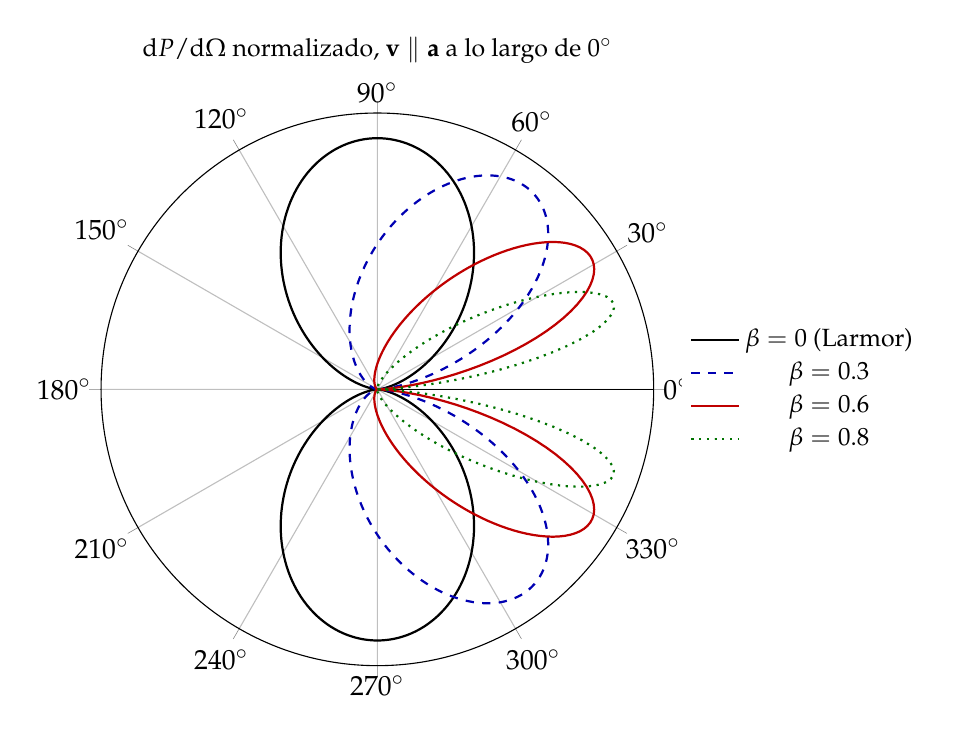
\begin{tikzpicture}
\begin{polaraxis}[width=8.6cm,
  xtick={0,30,...,330},ytick=\empty,
  xticklabel={$\pgfmathprintnumber{\tick}^\circ$},
  legend style={at={(1.05,0.5)},anchor=west,font=\small,draw=none},
  domain=0:360,samples=361,
  title={\small $\dd P/\dd\Omega$ normalizado, $\bv\parallel\av$ a lo largo de $0^\circ$}]
\addplot[black,thick,data cs=polar] (x,{sin(x)^2});
\addplot[blue!70!black,thick,dashed,data cs=polar] (x,{sin(x)^2/(1-0.3*cos(x))^5/1.72658});
\addplot[red!75!black,thick,data cs=polar] (x,{sin(x)^2/(1-0.6*cos(x))^5/9.82387});
\addplot[green!45!black,thick,dotted,data cs=polar] (x,{sin(x)^2/(1-0.8*cos(x))^5/124.0781});
\legend{$\beta=0$ (Larmor),$\beta=0.3$,$\beta=0.6$,$\beta=0.8$}
\end{polaraxis}
\end{tikzpicture}

{\small Figura 1. Lóbulos de radiación para $\av\parallel\bv$ (cada curva normalizada a su máximo).
Los máximos están en $90^\circ$, $53.7^\circ$, $31.8^\circ$ y $20.0^\circ$, de acuerdo con la fórmula
de $\theta_{\max}$. No hay emisión exactamente hacia adelante: $\sin^2\theta=0$ en $\theta=0$.}
\end{center}

\subsection{Aceleración perpendicular a la velocidad}

Se toma $\bbeta=\beta\hat{\mathbf z}$, $\av=a\hat{\mathbf x}$. Expandiendo con el doble producto vectorial,
$\nh\times(\uv\times\av)=\uv(\nh\cdot\av)-\av(\nh\cdot\uv)$:
\[
|\nh\times(\uv\times\av)|^2=u^2(\nh\cdot\av)^2-2(\nh\cdot\av)(\nh\cdot\uv)(\uv\cdot\av)+a^2(\nh\cdot\uv)^2.
\]
Se sustituye $\uv\cdot\av=c\,\nh\cdot\av$ (porque $\bbeta\cdot\av=0$), $u^2=c^2(1-2\beta\cos\theta+\beta^2)$,
$\nh\cdot\uv=c(1-\beta\cos\theta)$ y $\nh\cdot\av=a\sin\theta\cos\phi$:
\begin{align*}
\frac{|\cdot|^2}{c^2}
&=(\nh\cdot\av)^2\Big[1-2\beta\cos\theta+\beta^2-2(1-\beta\cos\theta)\Big]+a^2(1-\beta\cos\theta)^2\\
&=a^2\Big[(1-\beta\cos\theta)^2-(1-\beta^2)\sin^2\theta\cos^2\phi\Big].
\end{align*}
\begin{resbox}{Aceleración $\perp$ velocidad (movimiento circular, sincrotrón)}
\begin{equation}
\frac{\dd P}{\dd\Omega}=\frac{\mu_0q^2a^2}{16\pi^2c}\,
\frac{(1-\beta\cos\theta)^2-(1-\beta^2)\sin^2\theta\cos^2\phi}{(1-\beta\cos\theta)^5},
\qquad P=\frac{\mu_0q^2a^2\gamma^4}{6\pi c}.
\label{eq:perp}
\end{equation}
(Ej.~\ref{ej:perp})
\end{resbox}

% ================= 7 =================
\section{Radiación dipolar (Griffiths §11.1, Jackson §9.2)}

\subsection{Dipolo eléctrico oscilante}

Se considera $\mathbf p(t)=p_0\cos\omega t\,\hat{\mathbf z}$, con $p_0=q_0d$, formado por cargas
$\pm q_0\cos\omega t$ en $z=\pm d/2$. Aproximaciones:
\begin{center}
(i) $d\ll r$ (dipolo puntual),\qquad (ii) $d\ll\lambda=2\pi c/\omega$ (dipolo pequeño),\qquad
(iii) $r\gg\lambda$ (zona de radiación).
\end{center}

\textbf{Potencial escalar.} Por (i), $R_\pm\simeq r\left(1\mp\frac d{2r}\cos\theta\right)$ y
$\frac1{R_\pm}\simeq\frac1r\left(1\pm\frac d{2r}\cos\theta\right)$. Por (ii):
\[
\cos[\omega(t-R_\pm/c)]\simeq\cos[\omega(t-r/c)]\mp\frac{\omega d}{2c}\cos\theta\,\sin[\omega(t-r/c)].
\]
Con $C\equiv\cos[\omega(t-r/c)]$, $S\equiv\sin[\omega(t-r/c)]$, $\epsilon=\frac d{2r}\cos\theta$,
$\delta=\frac{\omega d}{2c}\cos\theta$:
\[
V=\frac{q_0}{4\pi\varepsilon_0r}\Big[(1+\epsilon)(C-\delta S)-(1-\epsilon)(C+\delta S)\Big]
=\frac{q_0}{4\pi\varepsilon_0r}\big[2\epsilon C-2\delta S\big]
=\frac{p_0\cos\theta}{4\pi\varepsilon_0r}\left[\frac{C}{r}-\frac{\omega}{c}S\right].
\]
El primer término es el dipolo estático; por (iii), $r\gg c/\omega$, domina el segundo:
\begin{equation}
V\simeq-\frac{p_0\omega}{4\pi\varepsilon_0c}\,\frac{\cos\theta}{r}\,\sin[\omega(t-r/c)].
\end{equation}

\textbf{Potencial vector.} $I(t)=\dot q=-q_0\omega\sin\omega t$, y la integral en
$z\in[-d/2,d/2]$ aporta un factor $d$:
\begin{equation}
\mathbf A\simeq-\frac{\mu_0p_0\omega}{4\pi r}\,\sin[\omega(t-r/c)]\,\hat{\mathbf z}.
\end{equation}

\textbf{Campos.} En zona de radiación sólo se conservan términos $1/r$, que provienen de derivar la
fase. Usando $1/(\varepsilon_0c^2)=\mu_0$ y $\hat{\mathbf z}=\cos\theta\,\hat{\mathbf r}-\sin\theta\,\hat{\bm\theta}$:
\[
\nabla V\simeq\frac{\partial V}{\partial r}\hat{\mathbf r}=\frac{\mu_0p_0\omega^2}{4\pi}\frac{\cos\theta}{r}C\,\hat{\mathbf r},
\qquad
-\frac{\partial\mathbf A}{\partial t}=\frac{\mu_0p_0\omega^2}{4\pi r}C\,(\cos\theta\,\hat{\mathbf r}-\sin\theta\,\hat{\bm\theta}).
\]
Las componentes radiales se cancelan. Para $\mathbf B$, con $A_\theta=-A\sin\theta$, domina
$\frac1r\partial_r(rA_\theta)$:
\begin{resbox}{Campos de radiación del dipolo eléctrico}
\begin{equation}
\mathbf E=-\frac{\mu_0p_0\omega^2}{4\pi}\frac{\sin\theta}{r}\cos[\omega(t-r/c)]\,\hat{\bm\theta},\qquad
\mathbf B=-\frac{\mu_0p_0\omega^2}{4\pi c}\frac{\sin\theta}{r}\cos[\omega(t-r/c)]\,\hat{\bm\phi}.
\end{equation}
Con $\hat{\bm\theta}\times\hat{\bm\phi}=\hat{\mathbf r}$ y $\langle\cos^2\rangle=\tfrac12$:
\begin{equation}
\langle\mathbf S\rangle=\frac{\mu_0p_0^2\omega^4}{32\pi^2c}\,\frac{\sin^2\theta}{r^2}\,\hat{\mathbf r},\qquad
\langle P\rangle=\frac{\mu_0p_0^2\omega^4}{12\pi c}.
\end{equation}
\end{resbox}
La dependencia $\omega^4$ es la de la dispersión de Rayleigh (cielo azul).

\subsection{Fuente arbitraria y dipolo magnético}

Para una distribución arbitraria de tamaño $\ll\lambda$ (Griffiths 11.1.4):
\begin{equation}
\mathbf E_{\rm rad}=\frac{\mu_0}{4\pi r}\Big[\hat{\mathbf r}\times(\hat{\mathbf r}\times\ddot{\mathbf p})\Big]_{t_0},\qquad
P=\frac{\mu_0\,\ddot p^2(t_0)}{6\pi c},\qquad t_0=t-r/c.
\end{equation}
Con $\ddot{\mathbf p}=q\av$ esto \emph{es} Larmor. Para un dipolo magnético $m_0\cos\omega t$:
$\langle P\rangle_{\rm mag}=\dfrac{\mu_0m_0^2\omega^4}{12\pi c^3}$; para una espira de radio $b$,
$P_{\rm mag}/P_{\rm el}=(\omega b/c)^2\ll1$.

% ================= 8 =================
\section{Reacción de radiación (Griffiths §11.2.2)}

Se busca $\mathbf F_{\rm rad}$ cuyo trabajo compense la energía radiada en un intervalo donde el estado
se repite ($\bv\cdot\av$ igual en $t_1$ y $t_2$). Integrando por partes:
\[
\int_{t_1}^{t_2}\mathbf F_{\rm rad}\cdot\bv\,\dd t=-\frac{\mu_0q^2}{6\pi c}\int_{t_1}^{t_2}\dot\bv\cdot\dot\bv\,\dd t
=-\frac{\mu_0q^2}{6\pi c}\left\{\big[\bv\cdot\dot\bv\big]_{t_1}^{t_2}-\int_{t_1}^{t_2}\ddot\bv\cdot\bv\,\dd t\right\}.
\]
El término de borde se anula, lo que permite identificar:
\begin{resbox}{Fórmula de Abraham--Lorentz}
\begin{equation}
\mathbf F_{\rm rad}=\frac{\mu_0q^2}{6\pi c}\,\dot\av,\qquad
\tau\equiv\frac{\mu_0q^2}{6\pi mc}=6.26\times10^{-24}\ \text{s (electrón)}.
\end{equation}
\end{resbox}
Sin fuerza externa, $\av=\tau\dot\av$ tiene la solución desbocada $\av=\av_0e^{t/\tau}$; eliminarla exige
preaceleración (violación de causalidad en escalas $\sim\tau$). Es un síntoma de que la electrodinámica
clásica de cargas puntuales falla a escalas $\sim c\tau\sim r_e$.

% ================= 9 =================
\section{Reglas y estrategias para resolver problemas}

\subsection{Qué herramienta usar según el tipo de problema}

\begin{center}
\renewcommand{\arraystretch}{1.3}
\begin{tabularx}{\textwidth}{>{\raggedright}p{6.3cm}>{\raggedright\arraybackslash}X}
\toprule
\textbf{Si el problema pide\ldots} & \textbf{Herramienta}\\
\midrule
Potenciales de una distribución $\rho(\rr,t)$, $\mathbf J(\rr,t)$ & Potenciales retardados \eqref{eq:retard}; determinar la región causal $t_r>0$.\\
Campos de una corriente que se enciende & $\mathbf A$ retardado, luego $\mathbf E=-\partial_t\mathbf A$, $\mathbf B=\nabla\times\mathbf A$ (Ej.~\ref{ej:alambre}).\\
Verificar que algo resuelve $\boxop\Psi=-4\pi f$ & Derivar a través de $t_r$: $\nabla t_r=-\hat{\mathbf R}/c$ (Ej.~\ref{ej:verif}).\\
Potenciales de una carga puntual & Liénard--Wiechert \eqref{eq:LW}; resolver $c(t-t_r)=|\rr-\mathbf w(t_r)|$.\\
Potencia total de una carga, $v\ll c$ & Larmor \eqref{eq:larmor}.\\
Potencia total, relativista & Liénard \eqref{eq:lienard}; casos $\parallel$: $\gamma^6$, $\perp$: $\gamma^4$.\\
Dirección de máxima emisión & Derivar $\dd P/\dd\Omega$ respecto de $\theta$ \eqref{eq:paralelo}.\\
Sistema oscilante pequeño ($d\ll\lambda$) & Dipolo: $P=\mu_0\ddot p^2/6\pi c$; promediar en el tiempo.\\
Superposición de dipolos desfasados & Sumar $\ddot{\mathbf p}$ \emph{antes} de elevar al cuadrado (Ej.~\ref{ej:rotante}).\\
Tiempo de decaimiento de una órbita & $\dd E/\dd t=-P$ con $E(r)$ y $a(r)$ de la órbita (Ej.~\ref{ej:hidrogeno}).\\
\bottomrule
\end{tabularx}
\end{center}

\subsection{Consideraciones y trucos}

\begin{enumerate}[itemsep=0.4em]
\item \textbf{Causalidad primero.} Antes de integrar, determina qué parte de la fuente ya alcanzó a
``hablar'' con el punto de observación: $t-R/c>t_{\rm encendido}$.
\item \textbf{Delta de una función.} $\delta(g(t'))=\sum_i\delta(t'-t_i)/|g'(t_i)|$. Es el origen del
factor $1-\Rh\cdot\bbeta$ en Liénard--Wiechert.
\item \textbf{$\dd t$ vs.\ $\dd t_r$.} La potencia \emph{emitida} usa $\dd W/\dd t_r$; la \emph{recibida},
$\dd W/\dd t$. Difieren en un factor $(1-\nh\cdot\bbeta)$: por eso aparece la quinta potencia y no la sexta.
\item \textbf{Zona de radiación.} Sólo los términos $1/r$ en los campos; se obtienen derivando la fase
$\omega(t-r/c)$, no la amplitud.
\item \textbf{Chequeos de límite.} $\beta\to0$ debe dar Larmor y $\sin^2\theta$; $t\to\infty$ en un
encendido debe dar el resultado estático; $\gamma\gg1$ concentra todo en un cono $\sim1/\gamma$.
\item \textbf{Misma fuerza, distinta pérdida.} Si $F\parallel v$, $F=\gamma^3ma$; si $F\perp v$,
$F=\gamma ma$. Por eso $P_\perp/P_\parallel=\gamma^2$ a fuerza igual.
\item \textbf{Promedios temporales.} $\langle\cos^2\rangle=\langle\sin^2\rangle=\tfrac12$,
$\langle\sin\cos\rangle=0$. No promedies amplitudes antes de elevarlas al cuadrado.
\end{enumerate}

\begin{warnbox}{Errores frecuentes}
\begin{itemize}[itemsep=0.2em,leftmargin=1.2em]
\item Retardar Coulomb en vez de los potenciales.
\item Olvidar que $\Rs$, $\bv$, $\av$ en \eqref{eq:LWfields} se evalúan en $t_r$, no en $t$.
\item Usar $\theta$ medido desde $\av$ en \eqref{eq:paralelo} cuando el enunciado lo mide desde $\bv$
(en ese caso coinciden, pero en \eqref{eq:perp} no).
\item En el dipolo, conservar términos $1/r^2$ en la zona de radiación.
\item Mezclar unidades gaussianas de Jackson Cap.~14 con SI.
\end{itemize}
\end{warnbox}

% ================= 10 =================
\newpage
\section{Ejercicios resueltos}

\ejercicio{Alambre infinito que se enciende (Griffiths Ej.~10.2)}\label{ej:alambre}
Un alambre infinito sobre el eje $z$ lleva $I(t)=0$ para $t<0$ e $I(t)=I_0$ para $t>0$. Encontrar
$\mathbf A$, $\mathbf E$ y $\mathbf B$ a distancia $s$.

\sol Un elemento en $z$ contribuye sólo si $t_r=t-\sqrt{s^2+z^2}/c>0$, es decir, si
$|z|<z_m\equiv\sqrt{c^2t^2-s^2}$, lo que exige $t>s/c$ (antes, $\mathbf A=0$). Entonces
\[
A_z=\frac{\mu_0I_0}{4\pi}\,2\int_0^{z_m}\frac{\dd z}{\sqrt{s^2+z^2}}
=\frac{\mu_0I_0}{2\pi}\ln\!\left(\frac{z_m+\sqrt{s^2+z_m^2}}{s}\right)
=\frac{\mu_0I_0}{2\pi}\ln\!\left(\frac{ct+\sqrt{c^2t^2-s^2}}{s}\right),
\]
usando $\sqrt{s^2+z_m^2}=ct$. Sea $k=\mu_0I_0/2\pi$ y $\Sigma=\sqrt{c^2t^2-s^2}$.

\textit{Campo eléctrico.}
\[
\partial_tA_z=k\,\frac{c+c^2t/\Sigma}{ct+\Sigma}=k\,\frac{c(\Sigma+ct)/\Sigma}{ct+\Sigma}=\frac{kc}{\Sigma}
\quad\Longrightarrow\quad
\boxed{\mathbf E=-\frac{\mu_0I_0c}{2\pi\sqrt{c^2t^2-s^2}}\,\hat{\mathbf z}}
\]

\textit{Campo magnético.} Usando $\Sigma^2=c^2t^2-s^2$ en el numerador:
\[
\partial_sA_z=k\left[\frac{-s/\Sigma}{ct+\Sigma}-\frac1s\right]
=-k\,\frac{s^2+ct\Sigma+\Sigma^2}{s\Sigma(ct+\Sigma)}
=-k\,\frac{ct(ct+\Sigma)}{s\Sigma(ct+\Sigma)}=-\frac{k\,ct}{s\Sigma},
\]
\[
\boxed{\mathbf B=-\partial_sA_z\,\hat{\bm\phi}=\frac{\mu_0I_0}{2\pi s}\,\frac{ct}{\sqrt{c^2t^2-s^2}}\,\hat{\bm\phi}}
\]
\textit{Chequeo:} $t\to\infty$ da $\mathbf E\to0$, $\mathbf B\to\mu_0I_0/(2\pi s)\,\hat{\bm\phi}$ (magnetostática).
En $t\to s/c^+$ ambos divergen: el frente de onda llega de golpe con el escalón de corriente.

\ejercicio{Los potenciales retardados resuelven la ecuación de onda}\label{ej:verif}
Verificar que $V$ de \eqref{eq:retard} satisface $\boxop V=-\rho/\varepsilon_0$.

\sol La dependencia en $\rr$ entra por $R$ y por $t_r$. Con $\nabla t_r=-\hat{\mathbf R}/c$:
\[
\nabla\rho(\rr',t_r)=\dot\rho\,\nabla t_r=-\frac{\dot\rho}{c}\hat{\mathbf R},\qquad
\nabla\frac1R=-\frac{\hat{\mathbf R}}{R^2}
\quad\Longrightarrow\quad
\nabla V=\frac1{4\pi\varepsilon_0}\int\left[-\frac{\dot\rho}{c}\frac{\hat{\mathbf R}}{R}-\rho\frac{\hat{\mathbf R}}{R^2}\right]\dd\tau'.
\]
Divergencia, con $\nabla\cdot(\hat{\mathbf R}/R)=1/R^2$, $\nabla\cdot(\hat{\mathbf R}/R^2)=4\pi\delta^{(3)}(\mathbf R)$,
$\nabla\dot\rho=-\ddot\rho\hat{\mathbf R}/c$, $\nabla\rho=-\dot\rho\hat{\mathbf R}/c$:
\begin{align*}
\nabla^2V&=\frac1{4\pi\varepsilon_0}\int\left[-\frac1c\left(-\frac{\ddot\rho}{c}\frac{\hat{\mathbf R}\cdot\hat{\mathbf R}}{R}+\frac{\dot\rho}{R^2}\right)
-\left(-\frac{\dot\rho}{c}\frac{\hat{\mathbf R}\cdot\hat{\mathbf R}}{R^2}+4\pi\rho\,\delta^{(3)}(\mathbf R)\right)\right]\dd\tau'\\
&=\frac1{4\pi\varepsilon_0}\int\left[\frac{\ddot\rho}{c^2R}-\frac{\dot\rho}{cR^2}+\frac{\dot\rho}{cR^2}-4\pi\rho\,\delta^{(3)}(\mathbf R)\right]\dd\tau'
=\frac1{c^2}\frac{\partial^2V}{\partial t^2}-\frac{\rho(\rr,t)}{\varepsilon_0}.\quad\checkmark
\end{align*}
Los términos en $\dot\rho$ se cancelan exactamente; el término en $\ddot\rho$ es $c^{-2}\partial_t^2V$
porque $\partial_t$ actúa sobre $\rho(\rr',t-R/c)$ como derivada respecto de $t_r$.

\ejercicio{Función de Green de la ecuación de onda en 1D}\label{ej:green1d}
Resolver $\left(\partial_x^2-\frac1{c^2}\partial_t^2\right)G=-\delta(x)\delta(t)$ con condición retardada.

\sol Fourier en $t$: $G''+k^2G_k=-\delta(x)$, $k=\omega/c$. Para $x\neq0$, $G_k=Ae^{ik|x|}$ (onda
saliente). La condición de salto es $G_k'(0^+)-G_k'(0^-)=-1$. Como $G_k'(0^\pm)=\pm ikA$, el salto es
$2ikA=-1$, de modo que $A=i/(2k)$:
\[
G_k(x)=\frac{i}{2k}e^{ik|x|}=\frac{ic}{2\omega}e^{i\omega|x|/c}.
\]
Volviendo al tiempo, con $s\equiv t-|x|/c$ y la prescripción retardada $\omega\to\omega+i\epsilon$:
\[
G(x,t)=\frac1{2\pi}\int\dd\omega\,\frac{ic}{2(\omega+i\epsilon)}e^{-i\omega s}.
\]
El polo está en $\omega=-i\epsilon$. Si $s<0$ se cierra por arriba y $G=0$. Si $s>0$ se cierra por
abajo (sentido horario): $\int\dd\omega\,\frac{e^{-i\omega s}}{\omega+i\epsilon}=-2\pi i$. Luego
\[
\boxed{G(x,t)=\frac{c}{2}\,\Theta\!\left(t-\frac{|x|}{c}\right)}
\]
\textit{Física:} en 1D la respuesta a un pulso \emph{no} es un pulso sino un escalón que persiste (``estela'').
En 3D es una cáscara $\delta(t-R/c)/R$: el principio de Huygens fuerte sólo vale en dimensión espacial
impar $\geq3$. Compárese con la Sec.~10 de los apuntes (1D, 2D, 3D estáticos).

\ejercicio{Potencial de una carga con velocidad constante (Griffiths Ej.~10.4)}\label{ej:vconst}
Una carga se mueve con $\mathbf w(t)=\bv t$. Encontrar $V(\rr,t)$.

\sol La condición de retardo $|\rr-\bv t_r|=c(t-t_r)$, al cuadrado, es
$r^2-2\rr\cdot\bv\,t_r+v^2t_r^2=c^2(t^2-2tt_r+t_r^2)$:
\[
(c^2-v^2)t_r^2-2(c^2t-\rr\cdot\bv)t_r+(c^2t^2-r^2)=0
\]
\[
\Rightarrow\quad t_r=\frac{(c^2t-\rr\cdot\bv)-\sqrt{(c^2t-\rr\cdot\bv)^2+(c^2-v^2)(r^2-c^2t^2)}}{c^2-v^2}.
\]
Se elige el signo $-$ porque con $v=0$ debe dar $t_r=t-r/c$. Ahora, con $\Rs=c(t-t_r)$ y
$\Rv\cdot\bv=\rr\cdot\bv-v^2t_r$:
\[
\begin{aligned}
\Rs c-\Rv\cdot\bv&=c^2t-c^2t_r-\rr\cdot\bv+v^2t_r=(c^2t-\rr\cdot\bv)-(c^2-v^2)t_r\\
&=\sqrt{(c^2t-\rr\cdot\bv)^2+(c^2-v^2)(r^2-c^2t^2)}.
\end{aligned}
\]
\[
\boxed{V(\rr,t)=\frac1{4\pi\varepsilon_0}\,\frac{qc}{\sqrt{(c^2t-\rr\cdot\bv)^2+(c^2-v^2)(r^2-c^2t^2)}}},\qquad\mathbf A=\frac{\bv}{c^2}V
\]
Todo quedó en función de $t$ (no de $t_r$): para movimiento uniforme el retardo se puede eliminar por
completo.

\ejercicio{Aceleración paralela: máximo y potencia total}\label{ej:paralelo}
\sol\textit{Máximo.} Se maximiza $f(\theta)=\sin^2\theta\,(1-\beta\cos\theta)^{-5}$:
\[
f'=\frac{2\sin\theta\cos\theta(1-\beta\cos\theta)-5\beta\sin^3\theta}{(1-\beta\cos\theta)^6}=0.
\]
Dividiendo por $\sin\theta$ y con $x=\cos\theta$, $\sin^2\theta=1-x^2$:
\[
2x(1-\beta x)-5\beta(1-x^2)=0\ \Longrightarrow\ 3\beta x^2+2x-5\beta=0
\ \Longrightarrow\ \boxed{\cos\theta_{\max}=\frac{\sqrt{1+15\beta^2}-1}{3\beta}}
\]
(raíz con $|x|\leq1$). Si $\beta\to0$, $\cos\theta_{\max}\simeq\frac{1+\frac{15}2\beta^2-1}{3\beta}=\frac52\beta\to0$:
$\theta_{\max}\to\pi/2$ (Larmor). Si $\gamma\gg1$, $\beta\simeq1-\frac1{2\gamma^2}$, $\sqrt{1+15\beta^2}\simeq4-\frac{15}{8\gamma^2}$ y
\[
\cos\theta_{\max}\simeq\left(1-\frac5{8\gamma^2}\right)\left(1+\frac1{2\gamma^2}\right)\simeq1-\frac1{8\gamma^2}
\equiv1-\frac{\theta_{\max}^2}{2}\ \Longrightarrow\ \theta_{\max}\simeq\frac1{2\gamma}.
\]

\textit{Total.} $\displaystyle\int\frac{\sin^2\theta}{(1-\beta\cos\theta)^5}\dd\Omega=2\pi\int_{-1}^1\frac{1-x^2}{(1-\beta x)^5}\dd x$.
Con $u=1-\beta x$, $x=(1-u)/\beta$, $\dd x=-\dd u/\beta$ y $1-x^2=[\beta^2-(1-u)^2]/\beta^2$:
\[
\begin{aligned}
\int_{-1}^1\frac{1-x^2}{(1-\beta x)^5}\dd x&=\frac1{\beta^3}\int_{1-\beta}^{1+\beta}\Big[-(1-\beta^2)u^{-5}+2u^{-4}-u^{-3}\Big]\dd u\\
&=\frac1{\beta^3}\left[\frac{1-\beta^2}{4u^4}-\frac2{3u^3}+\frac1{2u^2}\right]_{1-\beta}^{1+\beta}=\frac43\gamma^6.
\end{aligned}
\]
\[
P=\frac{\mu_0q^2a^2}{16\pi^2c}\cdot2\pi\cdot\frac43\gamma^6=\boxed{\frac{\mu_0q^2a^2\gamma^6}{6\pi c}}
\]
que coincide con Liénard \eqref{eq:lienard} con $\bv\times\av=0$.

\ejercicio{Aceleración perpendicular: potencia total y comparación}\label{ej:perp}
\sol Con $\int_0^{2\pi}\dd\phi=2\pi$ y $\int_0^{2\pi}\cos^2\phi\,\dd\phi=\pi$ en \eqref{eq:perp}:
\[
\int\dd\Omega\,[\cdots]=2\pi\int_{-1}^1\frac{\dd x}{(1-\beta x)^3}-\pi(1-\beta^2)\int_{-1}^1\frac{1-x^2}{(1-\beta x)^5}\dd x.
\]
Primera integral:
\[
\int_{-1}^1\frac{\dd x}{(1-\beta x)^3}=\left[\frac1{2\beta(1-\beta x)^2}\right]_{-1}^{1}
=\frac1{2\beta}\left[\frac1{(1-\beta)^2}-\frac1{(1+\beta)^2}\right]=\frac1{2\beta}\cdot\frac{4\beta}{(1-\beta^2)^2}=2\gamma^4.
\]
Segunda (Ej.~\ref{ej:paralelo}): $(1-\beta^2)\cdot\frac43\gamma^6=\frac43\gamma^4$. Suma:
$4\pi\gamma^4-\frac43\pi\gamma^4=\frac{8\pi}{3}\gamma^4$:
\[
\boxed{P_\perp=\frac{\mu_0q^2a^2\gamma^4}{6\pi c}}
\]
Con Liénard: $a^2-\beta^2a^2=a^2/\gamma^2$ y $\gamma^6/\gamma^2=\gamma^4$. \checkmark

\textit{A fuerza igual.} $F_\parallel=\gamma^3ma$, $F_\perp=\gamma ma$:
\[
P_\parallel=\frac{\mu_0q^2F^2}{6\pi cm^2},\qquad P_\perp=\frac{\mu_0q^2F^2}{6\pi cm^2}\gamma^2
\ \Longrightarrow\ \frac{P_\perp}{P_\parallel}=\gamma^2.
\]
\textit{Pérdida por vuelta (sincrotrón).} Con $a=\beta^2c^2/\rho$:
\[
\delta E=P_\perp\,\frac{2\pi\rho}{\beta c}=\frac{\mu_0q^2\beta^4c^3\gamma^4}{6\pi\rho^2}\cdot\frac{2\pi\rho}{\beta c}
=\frac{q^2\beta^3\gamma^4}{3\varepsilon_0\rho},
\]
que coincide con Jackson ec.~14.32 tras $q^2\to q^2/4\pi\varepsilon_0$.

\ejercicio{Dipolo rotante (Griffiths, Cap.~11)}\label{ej:rotante}
Dado $\mathbf p(t)=p_0(\cos\omega t\,\hat{\mathbf x}+\sin\omega t\,\hat{\mathbf y})$, encontrar
$\langle\mathbf S\rangle$ y $\langle P\rangle$.

\sol $\ddot{\mathbf p}=-\omega^2\mathbf p$. Con $\mathbf E_{\rm rad}=\frac{\mu_0}{4\pi r}\hat{\mathbf r}\times(\hat{\mathbf r}\times\ddot{\mathbf p})$:
\[
|\mathbf E_{\rm rad}|^2=\left(\frac{\mu_0}{4\pi r}\right)^2\Big[\ddot p^2-(\hat{\mathbf r}\cdot\ddot{\mathbf p})^2\Big],
\]
\[
\hat{\mathbf r}\cdot\mathbf p=p_0\sin\theta\,(\cos\phi\cos\omega t_0+\sin\phi\sin\omega t_0)=p_0\sin\theta\cos(\phi-\omega t_0).
\]
Promediando, $\langle\cos^2\rangle=\frac12$:
$\langle\ddot p^2-(\hat{\mathbf r}\cdot\ddot{\mathbf p})^2\rangle=\omega^4p_0^2\left(1-\frac12\sin^2\theta\right)=\omega^4p_0^2\,\frac{1+\cos^2\theta}{2}$.
\[
\langle\mathbf S\rangle=\frac{\langle E^2\rangle}{\mu_0c}\hat{\mathbf r}=\frac{\mu_0p_0^2\omega^4}{32\pi^2c}\,\frac{1+\cos^2\theta}{r^2}\,\hat{\mathbf r}.
\]
Con $\int(1+\cos^2\theta)\,\dd\Omega=4\pi+\frac{4\pi}{3}=\frac{16\pi}{3}$:
\[
\boxed{\langle P\rangle=\frac{\mu_0p_0^2\omega^4}{6\pi c}}
\]
el doble del dipolo lineal: superposición de dos dipolos en cuadratura (sin interferencia en el promedio).
Sobre el eje $z$ la radiación está polarizada circularmente; en el plano $xy$, linealmente.

\textit{Consistencia con Larmor.} Una carga $q$ en órbita circular de radio $R_0$ es un dipolo rotante con
$p_0=qR_0$; Larmor con $a=\omega^2R_0$ da $P=\mu_0q^2\omega^4R_0^2/(6\pi c)=\mu_0p_0^2\omega^4/(6\pi c)$. \checkmark

\ejercicio{Colapso clásico del átomo de hidrógeno}\label{ej:hidrogeno}
Un electrón está en órbita circular de radio $r_0=0.529$~Å. ¿En cuánto tiempo cae al núcleo?

\sol Órbita cuasi-circular:
\[
a=\frac{e^2}{4\pi\varepsilon_0mr^2},\qquad E=-\frac{e^2}{8\pi\varepsilon_0r}
\ \Rightarrow\ \frac{\dd E}{\dd t}=\frac{e^2}{8\pi\varepsilon_0r^2}\,\dot r.
\]
Igualando a $-P_{\rm Larmor}$ y usando $\mu_0=1/(\varepsilon_0c^2)$:
\[
\dot r=-\frac{8\pi\varepsilon_0r^2}{e^2}\cdot\frac{\mu_0e^2}{6\pi c}\cdot\frac{e^4}{16\pi^2\varepsilon_0^2m^2r^4}
=-\frac{e^4}{12\pi^2\varepsilon_0^2m^2c^3r^2}.
\]
Separando, $r^2\dd r=-\frac{e^4}{12\pi^2\varepsilon_0^2m^2c^3}\dd t$; integrando de $r_0$ a $0$:
\[
\boxed{t=\frac{4\pi^2\varepsilon_0^2m^2c^3r_0^3}{e^4}\approx1.6\times10^{-11}\ \text{s}}
\]
La física clásica no puede explicar la estabilidad atómica. La aproximación es consistente: $v/c\sim\alpha\approx1/137$
justifica Larmor no relativista y el cambio de $r$ por vuelta es pequeño.

% ================= 11 =================
\section{Ejercicios propuestos (con respuesta)}

\begin{enumerate}[label=\textbf{P\arabic*.},itemsep=0.6em,leftmargin=2.2em]
\item Muestre que $\frac12\left(G^{(+)}+G^{(-)}\right)$ también satisface \eqref{eq:defG}. ¿Qué
condición de contorno describe? \\
\textit{Resp.:} sí, por linealidad; describe ondas estacionarias (mitad entrante, mitad saliente), sin
pérdida neta de energía por radiación.

\item Una carga $q$ oscila como $z(t)=d\cos\omega t$ con $\omega d\ll c$. Calcule $\langle P\rangle$. \\
\textit{Resp.:} $\langle P\rangle=\dfrac{\mu_0q^2d^2\omega^4}{12\pi c}$ (Larmor con $\langle a^2\rangle=\frac12\omega^4d^2$, o dipolo con $p_0=qd$).

\item Demuestre que la \emph{resistencia de radiación} de un dipolo corto de longitud $d$ es
$R=\frac{2\pi}{3}\sqrt{\frac{\mu_0}{\varepsilon_0}}\left(\frac d\lambda\right)^2$. \\
\textit{Resp.:} con $p_0=I_0d/\omega$, $\langle P\rangle=\frac{\mu_0I_0^2d^2\omega^2}{12\pi c}\equiv\frac12RI_0^2$, de donde
$R\approx789\,(d/\lambda)^2\ \Omega$.

\item En \eqref{eq:perp}, encuentre las direcciones en el plano $\phi=0$ donde $\dd P/\dd\Omega=0$. \\
\textit{Resp.:} $\cos\theta=\beta$. Comprobación: $(1-\beta^2)^2-(1-\beta^2)(1-\beta^2)=0$.

\item Un electrón de $1$ GeV recorre un anillo de radio $\rho=10$ m. Estime la energía perdida por vuelta. \\
\textit{Resp.:} $\gamma=1957$, $\delta E=\frac{e^2\gamma^4}{3\varepsilon_0\rho}\approx8.9$ keV
(Jackson: $\delta E[\text{MeV}]=8.85\times10^{-2}\,E^4[\text{GeV}]/\rho[\text{m}]$).

\item Calcule $\langle P\rangle$ de un dipolo magnético $\mathbf m=m_0\cos\omega t\,\hat{\mathbf z}$ y compare
con un dipolo eléctrico de igual tamaño $b$. \\
\textit{Resp.:} $\langle P\rangle=\dfrac{\mu_0m_0^2\omega^4}{12\pi c^3}$; con $m_0=\pi b^2I_0$, $p_0=q_0b$:
$P_{\rm mag}/P_{\rm el}=(\omega b/c)^2$.

\item Para el alambre del Ej.~\ref{ej:alambre}, verifique que se cumple el gauge de Lorenz. \\
\textit{Resp.:} $V=0$ (alambre neutro) y $\nabla\cdot\mathbf A=\partial_zA_z=0$. \checkmark

\item Estime el tiempo característico de Abraham--Lorentz para un protón. \\
\textit{Resp.:} $\tau_p=\tau_e\,m_e/m_p\approx3.4\times10^{-27}$ s.
\end{enumerate}

\vspace{1em}
\begin{resbox}{Formulario mínimo para el quiz}
\begin{tabularx}{\linewidth}{>{\raggedright}p{4.2cm}X}
Green retardada & $G^{(+)}=\delta(t'-t+R/c)/R$,\quad $\boxop G=-4\pi\delta^{(3)}\delta$\\[0.3em]
Potenciales retardados & $V=\frac1{4\pi\varepsilon_0}\int\frac{\rho(t_r)}{R}\dd\tau'$,\quad $\mathbf A=\frac{\mu_0}{4\pi}\int\frac{\mathbf J(t_r)}{R}\dd\tau'$\\[0.3em]
Liénard--Wiechert & $V=\frac{1}{4\pi\varepsilon_0}\frac{qc}{\Rs c-\Rv\cdot\bv}$,\quad $\mathbf A=\bv V/c^2$\\[0.3em]
Larmor & $P=\mu_0q^2a^2/6\pi c$,\quad $\dd P/\dd\Omega\propto\sin^2\theta$\\[0.3em]
Liénard & $P=\frac{\mu_0q^2\gamma^6}{6\pi c}\left(a^2-|\bv\times\av|^2/c^2\right)$;\quad $\parallel$: $\gamma^6$,\ $\perp$: $\gamma^4$\\[0.3em]
Distribución angular & denominador $(1-\beta\cos\theta)^5$;\quad cono $\sim1/\gamma$\\[0.3em]
Dipolo eléctrico & $\langle P\rangle=\mu_0p_0^2\omega^4/12\pi c$,\quad patrón $\sin^2\theta$\\[0.3em]
Abraham--Lorentz & $\mathbf F=\mu_0q^2\dot\av/6\pi c$
\end{tabularx}
\end{resbox}

\end{document}
